% General introduction (Chapter 1). No \basedon: it is not based on a paper.
\chapter{General Introduction}

% chapterabstract with an empty heading: the text sits on the grey spread
% without an "Abstract" title. Use it for an opening passage.
\begin{chapterabstract}[]
[An opening passage for the thesis. It is set on its own page, facing a grey left-hand page.]

[A second paragraph.]
\end{chapterabstract}

\section{First Section of the Introduction}
[Introductory text. Cite with \verb|\citep| or \verb|\citet|: e.g. \citep{placeholderArticle2024} or \citet{placeholderBook2020}.]

\begin{figure}[htbp]
	\centering
	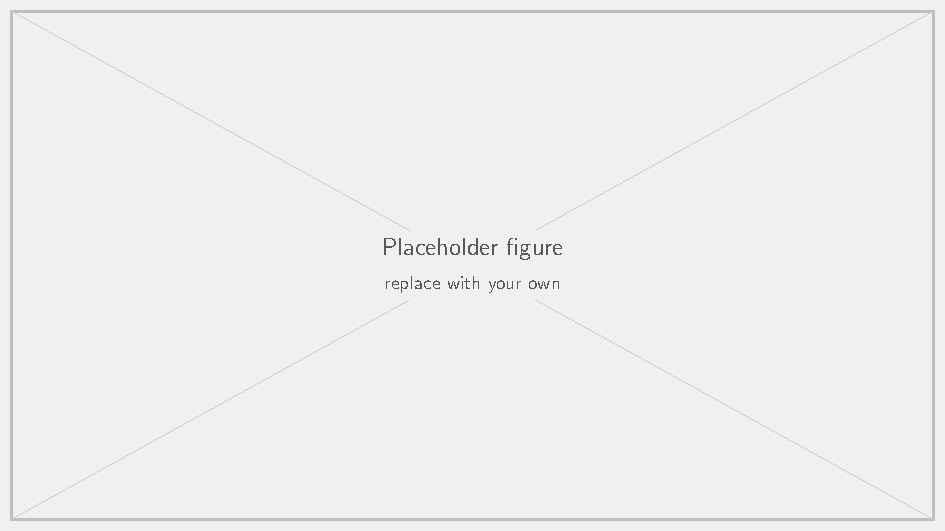
\includegraphics[width=\textwidth]{figures/placeholder.pdf}
	\caption{\textbf{Figure title.} Caption text. Figures shared by the introduction and discussion live in \texttt{figures/}.}
	\label{fig:intro-placeholder}
\end{figure}

\subsection{A Subsection}
[Text. Equations are numbered per chapter:]
\begin{equation}
	\frac{dz}{dt} = (a + i\omega)\,z - |z|^2 z .
	\label{eq:intro-example}
\end{equation}

\subsection{Another Subsection}
[Text referring to Figure~\ref{fig:intro-placeholder} and Equation~\ref{eq:intro-example}.]

\section{Second Section of the Introduction}
[Text.]

\section{Thesis Overview}
[Chapter~2 \ldots]

[Chapter~3 \ldots]

[Chapter~4 \ldots]

[Finally, Chapter~5 synthesises \ldots]
